\documentclass[tikz,border=2pt]{standalone}
\usepackage{amsmath,amssymb}
\usepackage{tikz}
\usetikzlibrary{arrows.meta}

\begin{document}
% A permutation is a bijection of a finite set onto itself: here pi = (1 3 4 2) on {1,2,3,4},
% drawn as an arrow diagram.
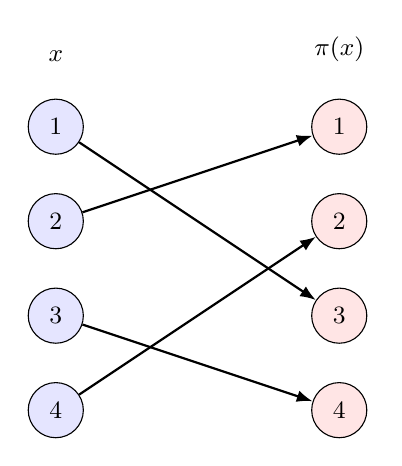
\begin{tikzpicture}[every node/.style={font=\small}, >={Latex[length=2mm]}]
	\foreach \i in {1,...,4} {
		\node[draw, circle, fill=blue!10, minimum size=7mm] (a\i) at (0,{3.6-1.2*\i}) {$\i$};
		\node[draw, circle, fill=red!10, minimum size=7mm] (b\i) at (3.6,{3.6-1.2*\i}) {$\i$};
	}
	\draw[->, thick] (a1) -- (b3);
	\draw[->, thick] (a2) -- (b1);
	\draw[->, thick] (a3) -- (b4);
	\draw[->, thick] (a4) -- (b2);
	\node[anchor=south] at (0,3.1) {$x$};
	\node[anchor=south] at (3.6,3.1) {$\pi(x)$};
\end{tikzpicture}
\end{document}
